
\documentclass[a4paper,11pt]{article}
\usepackage[a4paper, margin=8em]{geometry}

% usa i pacchetti per la scrittura in italiano
\usepackage[french,italian]{babel}
\usepackage[T1]{fontenc}
\usepackage[utf8]{inputenc}
\frenchspacing 

% usa i pacchetti per la formattazione matematica
\usepackage{amsmath, amssymb, amsthm, amsfonts}

% usa altri pacchetti
\usepackage{gensymb}
\usepackage{hyperref}
\usepackage{standalone}

% imposta il titolo
\title{Appunti Elettronica Digitale}
\author{Luca Seggiani}
\date{2026}

% imposta lo stile
% usa helvetica
\usepackage[scaled]{helvet}
% usa palatino
\usepackage{palatino}
% usa un font monospazio guardabile
\usepackage{lmodern}

\renewcommand{\rmdefault}{ppl}
\renewcommand{\sfdefault}{phv}
\renewcommand{\ttdefault}{lmtt}

% disponi il titolo
\makeatletter
\renewcommand{\maketitle} {
	\begin{center} 
		\begin{minipage}[t]{.8\textwidth}
			\textsf{\huge\bfseries \@title} 
		\end{minipage}%
		\begin{minipage}[t]{.2\textwidth}
			\raggedleft \vspace{-1.65em}
			\textsf{\small \@author} \vfill
			\textsf{\small \@date}
		\end{minipage}
		\par
	\end{center}

	\thispagestyle{empty}
	\pagestyle{fancy}
}
\makeatother

% disponi teoremi
\usepackage{tcolorbox}
\newtcolorbox[auto counter, number within=section]{theorem}[2][]{%
	colback=blue!10, 
	colframe=blue!40!black, 
	sharp corners=northwest,
	fonttitle=\sffamily\bfseries, 
	title=~\thetcbcounter: #2, 
	#1
}

% disponi definizioni
\newtcolorbox[auto counter, number within=section]{definition}[2][]{%
	colback=red!10,
	colframe=red!40!black,
	sharp corners=northwest,
	fonttitle=\sffamily\bfseries,
	title=~\thetcbcounter: #2,
	#1
}

% U.D.M
\newcommand{\amp}{\ensuremath{\mathrm{A}}}
\newcommand{\volt}{\ensuremath{\mathrm{V}}}
\newcommand{\meter}{\ensuremath{\mathrm{m}}}
\newcommand{\second}{\ensuremath{\mathrm{s}}}
\newcommand{\farad}{\ensuremath{\mathrm{F}}}
\newcommand{\henry}{\ensuremath{\mathrm{H}}}
\newcommand{\siemens}{\ensuremath{\mathrm{S}}}

% circuiti
\usepackage{circuitikz}
\usetikzlibrary{babel}

% disegni
\usepackage{pgfplots}
\pgfplotsset{width=10cm,compat=1.9}

% disponi codice
\usepackage{listings}
\usepackage[table]{xcolor}

\definecolor{codegreen}{rgb}{0,0.6,0}
\definecolor{codegray}{rgb}{0.5,0.5,0.5}
\definecolor{codepurple}{rgb}{0.58,0,0.82}
\definecolor{backcolour}{rgb}{0.95,0.95,0.92}

\lstdefinestyle{codestyle}{
		backgroundcolor=\color{black!5}, 
		commentstyle=\color{codegreen},
		keywordstyle=\bfseries\color{magenta},
		numberstyle=\sffamily\tiny\color{black!60},
		stringstyle=\color{green!50!black},
		basicstyle=\ttfamily\footnotesize,
		breakatwhitespace=false,         
		breaklines=true,                 
		captionpos=b,                    
		keepspaces=true,                 
		numbers=left,                    
		numbersep=5pt,                  
		showspaces=false,                
		showstringspaces=false,
		showtabs=false,                  
		tabsize=2
}

\lstdefinestyle{shellstyle}{
		backgroundcolor=\color{black!5}, 
		basicstyle=\ttfamily\footnotesize\color{black}, 
		commentstyle=\color{black}, 
		keywordstyle=\color{black},
		numberstyle=\color{black!5},
		stringstyle=\color{black}, 
		showspaces=false,
		showstringspaces=false, 
		showtabs=false, 
		tabsize=2, 
		numbers=none, 
		breaklines=true
}

\lstdefinelanguage{javascript}{
	keywords={typeof, new, true, false, catch, function, return, null, catch, switch, var, if, in, while, do, else, case, break},
	keywordstyle=\color{blue}\bfseries,
	ndkeywords={class, export, boolean, throw, implements, import, this},
	ndkeywordstyle=\color{darkgray}\bfseries,
	identifierstyle=\color{black},
	sensitive=false,
	comment=[l]{//},
	morecomment=[s]{/*}{*/},
	commentstyle=\color{purple}\ttfamily,
	stringstyle=\color{red}\ttfamily,
	morestring=[b]',
	morestring=[b]"
}

% disponi sezioni
\usepackage{titlesec}

\titleformat{\section}
	{\sffamily\Large\bfseries} 
	{\thesection}{1em}{} 
\titleformat{\subsection}
	{\sffamily\large\bfseries}   
	{\thesubsection}{1em}{} 
\titleformat{\subsubsection}
	{\sffamily\normalsize\bfseries} 
	{\thesubsubsection}{1em}{}

% disponi alberi
\usepackage{forest}

\forestset{
	rectstyle/.style={
		for tree={rectangle,draw,font=\large\sffamily}
	},
	roundstyle/.style={
		for tree={circle,draw,font=\large}
	}
}

% disponi algoritmi
\usepackage{algorithm}
\usepackage{algorithmic}
\makeatletter
\renewcommand{\ALG@name}{Algoritmo}
\makeatother

% disponi numeri di pagina
\usepackage{fancyhdr}
\fancyhf{} 
\fancyfoot[L]{\sffamily{\thepage}}

\makeatletter
\fancyhead[L]{\raisebox{1ex}[0pt][0pt]{\sffamily{\@title \ \@date}}} 
\fancyhead[R]{\raisebox{1ex}[0pt][0pt]{\sffamily{\@author}}}
\makeatother

\begin{document}
% sezione (data)
\section{Lezione del 21-04-26}

% stili pagina
\thispagestyle{empty}
\pagestyle{fancy}

% testo
\subsection{Risposta in frequenza}
Nel nostro studio dei componenti e circuiti elettronici abbiamo finora trascurato la risposta in \textbf{frequenza}. La risposta in frequenza è una grandezza che può effettivamente essere calcolata per circuiti, in quanto questi possono essere intesi come sistemi dinamici con una loro \textit{funzione di trasferimento} $H(s)$ nel dominio di Laplace:
$$
H(s) = \frac{V_u(s)}{V_i(s)}
$$

Per fare un esempio, prendiamo il circuito amplificatore MOSFET invertente a source comune, con capacità di accoppiamento al source, al gate e al drain. 

% circuito analizzato

Come sappiamo, ogni volta che introduciamo un condensatore o un induttore in un circuito, otteniamo un comportamento (propriamente un \textit{impedenza}) che dipende dalla frequenza o dalla pulsazione:
$$
Z_C = \frac{1}{j \omega C}, \quad Z_L = j \omega L, \quad \omega = 2 \pi f
$$

Ci interessa la risposta dell'amplificatore al piccolo segnale, per cui prendiamo il modello ai piccoli segnali:

% circuito equivalente

Notiamo che ad ogni MOSFET reale corrispondono capacità interne, o \textit{intrinseche}, cioè una $C_{GD}$ fra gate e drain, e una $C_{GS}$ fra gate e source. Queste andranno incluse nel modello, ed andranno a collegare lo stage di ingresso allo stage di uscita dell'amplificatore.

Solitamente, però, le capacità nel nostro circuito differiscono di diversi ordini di grandezza:
\begin{itemize}
	\item Le capacità $C_I$, $C_D$ e $C_S$ di accoppiamento saranno nell'ordine dei $\mu F$ o $n F$, cioè dai $10^{-6}$ ai $10^{-9}$ Farad;
	\item Le capacità $C_{GS}$ e $C_{GD}$ interne al MOSFET saranno nell'ordine dei $n F$ o $p F$, cioè dai $10^{-9}$ ai $10^{-12}$ Farad.
\end{itemize}

Spesso per questo motivo dividiamo le analisi in:
\begin{itemize}
	\item \textit{Bassa frequenza}, dove si considerano i condensatori esterni ($C_I$, $C_D$ e $C_S$) come attivi, e i condensatori intrinseci del MOSFET come circuiti aperti;

\begin{figure}[H]
\centering
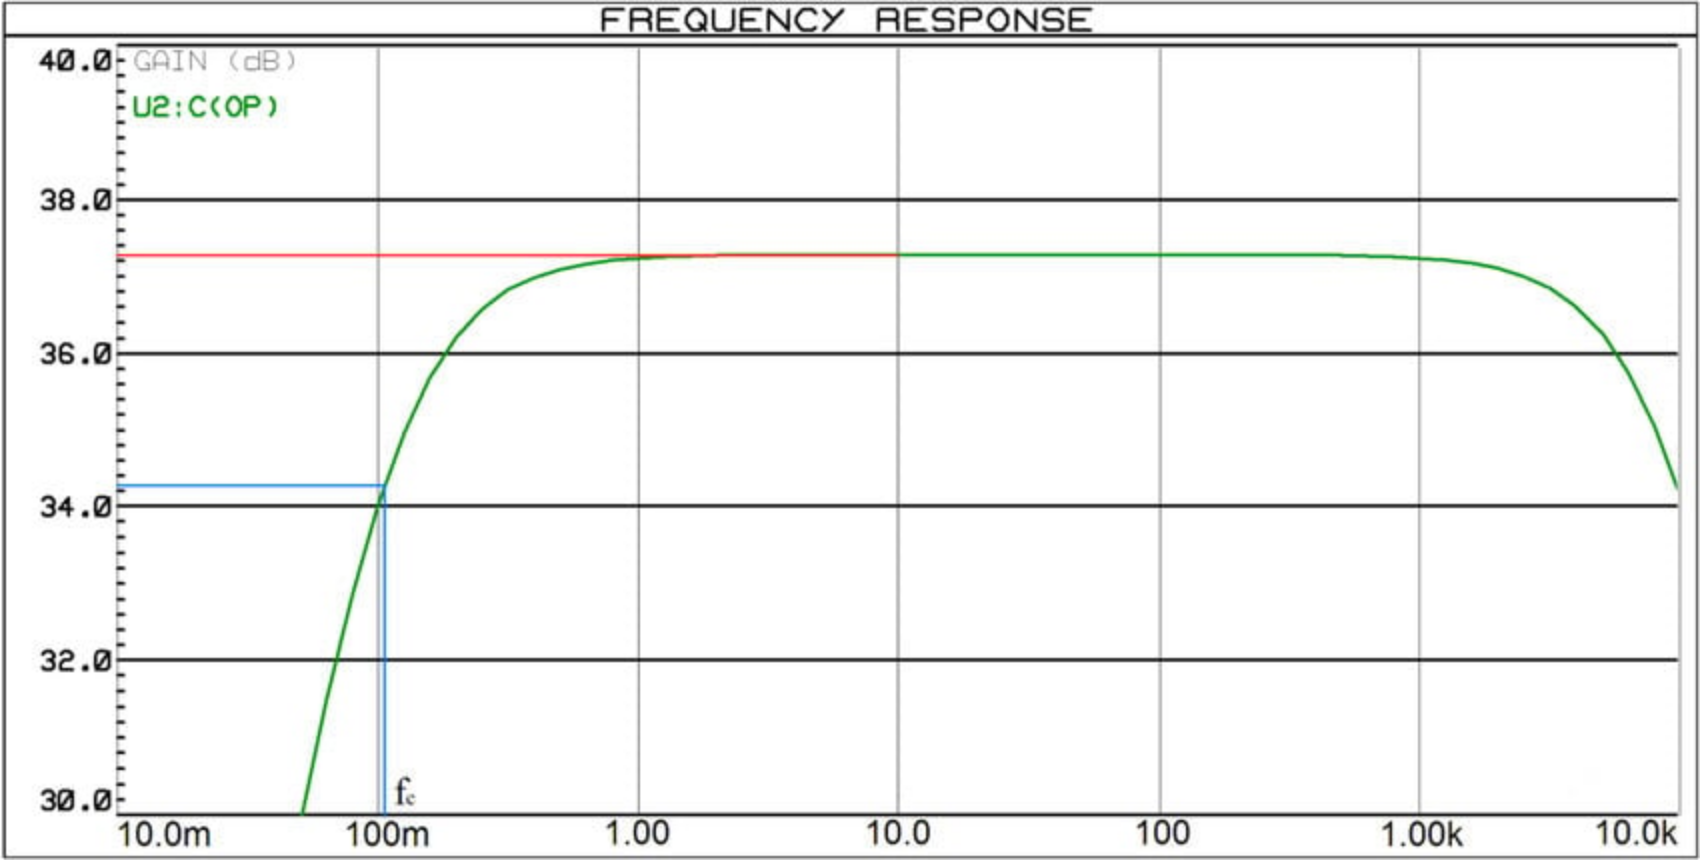
\includegraphics[width=0.48\textwidth]{../figures/ac_couple.png}
\hfill
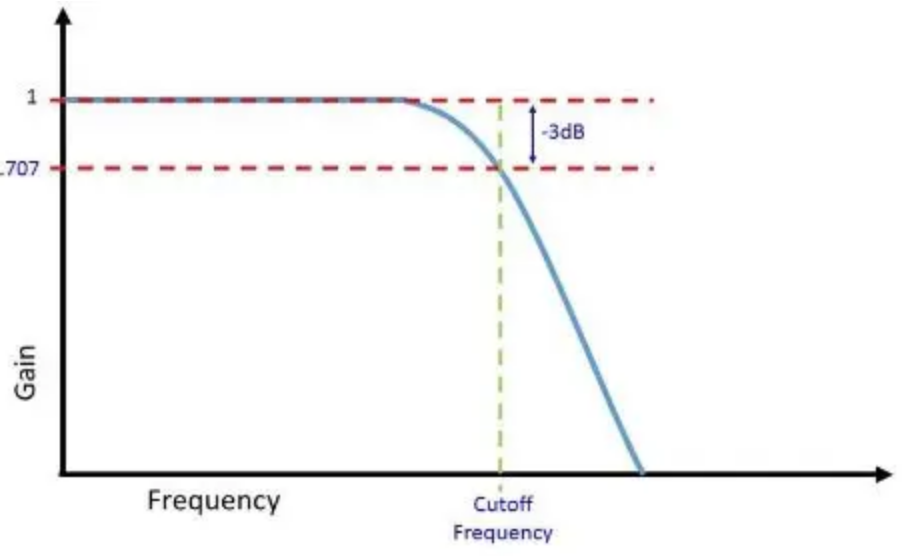
\includegraphics[width=0.48\textwidth]{../figures/dc_couple.png}
\end{figure}

	\item \textit{Media frequenza}, dove si considerano i condenstatori esterni come cortocircuiti, e i condensatori intrinseci come circuiti aperti. Chiamiamo questa zona \textit{centro banda}, dove abbiamo la risposta in \textit{accoppiamento AC} che ci interessa da un circuito. 

		Individuiamo sul centro banda le frequenze $f_L$ (\textit{limite inferiore} di centro banda) e $f_H$ (\textit{limite superiore} di centro banda), definite come la banda a $-3 \mathrm{dB}$ della risposta in frequenza. Esistono poi particolari circuiti dove si ha una banda centrata sull'$f_0 = 0$, e di cui individuiamo solo il \textit{limite superiore} di banda. Chiamiamo questi circuiti \textit{accoppiati in DC}.

	\item \textit{Alta frequenza}, dove si considerano i condensatori esterni come corto circuiti, e i condensatori intrinseci come attivi.
\end{itemize}

La zona di centro banda è quella dove il circuito amplificatore, ad esempio, ha caratteristiche lineari e costanti al variare della frequenza. Ad esempio, se si hanno $100 \mathrm{dB}$ di guadagno a centro banda, qualsiasi frequenza compresa fra $f_L$ e $f_H$ avrà (circa) tale guadagno, mentre a $f_L$ e $f_H$ avremo $97 \mathrm{dB}$ (dai $-3 \mathrm{dB}$ di banda).

In altri circuiti come ad esempio i \textit{filtri}, il guadagno avrà un decadimento lungo il centro banda del circuito (che sarà corrispondente alle caratteristiche del filtro, a $-12 \mathrm{dB}$, $-24 \mathrm{dB}$, ecc...). 

\newpage

Per ulteriori informazioni riguardo alla risposta in frequenza, il dominio di Laplace, i diagrammi di Bode, ecc... si rimanda agli appunti \url{https://raw.githubusercontent.com/seggiani-luca/appunti-et/e63e7e9ac9d57bd7b3f690140c8b460d91e0b08e/master/master.pdf} (elettrotecnica) e \url{https://raw.githubusercontent.com/seggiani-luca/appunti-ct/0ebb34499894cba25561c0b7a7bbf3db1cf0147b/master/master.pdf} (automatica).

\subsection{Teoria della reazione}
Alcuni dei circuiti che studiamo in elettronica sono \textit{instabili}, cioè hanno un comportamento che si evolve nel tempo in maniera incontrollata o comunque non costante. Ad esempio, questi possono essere gli \textit{oscillatori}, i \textit{flip-flop}, ecc...

La teoria che studia questo tipo di circuiti è la \textbf{teoria della reazione}, che vediamo adesso in maniera semplificata. Quello che prendiamo ad esempio è un circuito chiuso formato da:
\begin{itemize}
	\item Un \textit{amplificatore di segnale} $ A$;
	\item Una \textit{rete prelevatrice} che preleva il segnale in uscita dall'amplificatore. Da questa esce il segnale che va a carico della resistenza $R_L$;

		La rete prelevatrice può essere di 2 tipi: può infatti prelevare in \textit{tensione}, e prelevare in \textit{corrente};
	\item Una \textit{rete di reazione} $\beta$, anch'essa collegata all'uscita della rete prelevatrice, che elabora il segnale in uscita dall amplificatore;
	\item Una \textit{rete sommatrice} a monte dell'amplificatore, che somma il segnale dalla rete di reazione ad un altro segnale in ingresso $V_S$ (con associata resistenza $R_S$), e lo manda in ingresso all'amplificatore.

		La rete sommatrice può essere di 2 tipi: ad \textit{inserzione in serie}, e ad \textit{inserzione in parallelo}.
\end{itemize}

\begin{center}
\begin{tikzpicture}[transform shape]
	% Paths, nodes and wires:
	\node[shape=rectangle, draw, line width=1pt, minimum width=1.965cm, minimum height=1.965cm] at (5, 5){} node[anchor=center, align=center, text width=1.577cm, inner sep=6pt] at (5, 5){A};
	\node[shape=rectangle, draw, line width=1pt, minimum width=1.965cm, minimum height=1.965cm] at (9, 5){} node[anchor=center, align=center, text width=1.577cm, inner sep=6pt] at (9, 5){I};
	\node[shape=rectangle, draw, line width=1pt, minimum width=1.965cm, minimum height=1.965cm] at (5, 2){} node[anchor=center, align=center, text width=1.577cm, inner sep=6pt] at (5, 2){$\beta$};
	\draw (6, 5.5) -- (8, 5.5);
	\draw (6, 4.5) -- (8, 4.5);
	\draw (10, 5.5) -- (12, 5.5);
	\draw (10, 4.5) -- (12, 4.5);
	\draw (12, 5.5) to[american resistor, /tikz/circuitikz/bipoles/length=0.700cm, l={$R_L$}] (12, 4.5);
	\draw (6, 1.5) -| (9.5, 4);
	\draw (8.5, 4) |- (6, 2.5);
	\node[shape=rectangle, draw, line width=1pt, minimum width=1.965cm, minimum height=1.965cm] at (1, 5){} node[anchor=center, align=center, text width=1.577cm, inner sep=6pt] at (1, 5){+};
	\draw (4, 2.5) -| (1.5, 4);
	\draw (4, 1.5) |- (0.5, 1.5) -| (0.5, 4);
	\draw (2, 5.5) -- (4, 5.5);
	\draw (2, 4.5) -- (4, 4.5);
	\draw (-2, 4.5) -- (-0, 4.5);
	\draw (-2, 5.5) to[voltage source, /tikz/circuitikz/bipoles/length=0.700cm, l_={$V_i$}] (-2, 4.5);
	\draw (-2, 5.5) to[american resistor, /tikz/circuitikz/bipoles/length=0.700cm, l={$R_s$}] (0, 5.5);
\end{tikzpicture}
\end{center}

I tipi di rete prelevatrice e di rete di reazione sono caratteristiche ortogonali, per cui complessivamente abbiamo 4 tipologie di reti a reazione possibili.

Le semplificazioni che facciamo nello studio della reazione sono 3:
\begin{enumerate}
	\item Prendiamo l'amplificatore $A$ come \textit{unidirezionale}: questo significa che il segnale può passare solo nella direzione da sinistra a destra (dalla rete sommatrice alla rete di prelievo);
	\item Allo stesso modo, la rete di reazione $\beta$ sarà anch'essa unidirezionale: questo significa che il segnale può passare solo nella direzione da destra a sinistra (dalla rete di prelievo alla rete sommatrice);
	\item Infine, assumeremo che il valore della rete di reazione $\beta$ non dipende dal $R_S$ o da $R_L$, cioè né dal carico che dalla sorgente di segnale. 
\end{enumerate}
Fatte queste 3 ipotesi, studiare il sistema così formato diventa semplice. Altrimenti chiaramente vale il contrario. Notiamo che non è sempre il caso che una rete sia unidirezionale: in termini elettronici, nulla vieta che il segnale passi attraverso la rete di reazione, dall'ingresso all'uscita del circuito, senza effettuare il feedback dall'amplificatore.

Possiamo quindi semplificare il circuito di cui sopra al seguente schema a blocchi:

\begin{center}
\begin{tikzpicture}[transform shape]
	% Paths, nodes and wires:
	\node[shape=rectangle, draw, line width=1pt, minimum width=1.965cm, minimum height=1.965cm] at (5, 5.5){} node[anchor=center, align=center, text width=1.577cm, inner sep=6pt] at (5, 5.5){A};
	\node[shape=rectangle, draw, line width=1pt, minimum width=1.965cm, minimum height=1.965cm] at (5, 2){} node[anchor=center, align=center, text width=1.577cm, inner sep=6pt] at (5, 2){$\beta$};
	\draw (11, 5.5) to[american resistor, /tikz/circuitikz/bipoles/length=0.700cm, l={$R_L$}] (11, 4.5);
	\draw (-1.39, 5.485) to[american voltage source, /tikz/circuitikz/bipoles/length=0.700cm, l_={$V_i$}] (-1.39, 4.485);
	\draw (-1.39, 5.485) to[american resistor, /tikz/circuitikz/bipoles/length=0.700cm, l={$R_s$}] (0.61, 5.485);
	\node[shape=circle, draw, line width=1pt, minimum width=0.715cm](N1) at (0.985, 5.485){} node[anchor=center] at (N1.text){$+$};
	\draw (1.36, 5.485) -| (4, 5.5);
	\draw (4, 2) -| (0.985, 5.11);
	\draw (6, 5.5) -- (11, 5.5);
	\draw (9, 5.5) |- (6, 2);
	\node[tlground] at (-1.39, 4.485){};
	\node[tlground] at (11, 4.5){};
	\draw[-latex] (3.75, 6.75) -- (6.25, 6.75);
	\draw[-latex] (6.25, 3.25) -- (3.75, 3.25);
\end{tikzpicture}
\end{center}

dove gli unici elementi funzionali rimasti sono l'amplificatore $A$, la rete di reazione $\beta$, e il sommatore (che modellizza la rete sommatrice).
Di questa vorremo calcolare la funzione di trasferimento $H(s)$ come:
$$
H(s) = \frac{X_O(s)}{X_S(s)} = \frac{A(s)}{1 - \beta(s)A(s)}
$$
dal classico risultato di automatica:
$$
X_O = A X_I, \quad X_F = \beta X_O = \beta A X_F \implies X_I = X_S + X_F = X_S + \beta X_O
$$
$$
\implies X_O = A \left( X_S + \beta X_O \right) \implies (1 - \beta A) X_O = A X_S
$$
dove notiamo che prendiamo la convenzione col segno $-$ al denominatore, derivante dal fatto che sommiamo il segnale di feedback all'ingresso dell'amplificatore (al contrario della convenzione di automatica, in feedback negativo).

Chiamiamo i parametri individuati:
\begin{itemize}
	\item $A$: guadagno ad anello aperto;
	\item $\beta A$: guadagno di anello;
	\item $H$: guadagno ad anello chiuso. In particolare, distinfuiamo il tipo di reazione sulla base del rapporto fra $H$ e $A$:
		\begin{itemize}
			\item Se $|H| < |A|$ si parla di \textit{reazione negativa};
			\item Se $|H| > |A|$ si parla di \textit{reazione positiva}.
		\end{itemize}
\end{itemize}

Ci potremmo interrogare riguardo a come mai abbiamo bisogno di reazione negativa nei circuiti. La risposta si ha prendendo il limite per il guadagno ad anelo aperto che tende ad infinito:
$$
\lim_{A \rightarrow \infty} H = \lim_{A \rightarrow \infty} \frac{A}{1 - \beta A} = - \frac{1}{\beta}
$$
Questo significa che, nel caso di reazione stabile, il comportamento della rete è perfettamente predicibile e determinato dalla rete di reazione, qualsiasi siano le caratteristiche dell'amplificatore. Questo è utile ad esempio per gli amplificatori operazionli, che hanno guadagni $G_{OL}$ esorbitanti, ma diventano utili solo nel caso in cui si fornisce una rete stabilizzatrice in feedback che modula il guadagno a valori deterministici e costanti.

\subsubsection{Effetto del prelievo sull'impedenza}
Prendiamo l'esempio del prelievo di segnale in tensione all'uscita dell'amplificatore.

\begin{center}
\begin{tikzpicture}[transform shape]
	% Paths, nodes and wires:
	\draw (0, 6) to[american controlled voltage source, l={$A X_I$}] (0, 4);
	\draw (0, 6) to[american resistor, l={$R_O$}] (4, 6);
	\node[shape=rectangle, draw, line width=1pt, minimum width=1.965cm, minimum height=1.965cm] at (1, 1){} node[anchor=center, align=center, text width=1.577cm, inner sep=6pt] at (1, 1){$\beta$};
	\draw (3, 6) |- (2, 1.5);
	\draw (0, 4) -- (4, 4);
	\draw (3.5, 4) |- (2, 0.5);
	\draw (4, 6) to[open, o-o, l={$R_{of}$}] (4, 4);
	\node[circ] at (3, 6){};
	\node[circ] at (3.5, 4){};
\end{tikzpicture}
\end{center}

A questo punto potremmo interrogarci sulla resistenza $R_{of}$ in uscita dalla rete (assumendo una resistenza $R_o$ in uscita dall'amplificatore $A$). Ricordiamo da elettrotecnica che questa è data dal rapporto fra la tensione in circuito aperto $V_{oc}$ e la corrente in corto circuito $I_{cc}$:
$$
R_{of} = \frac{V_{oc}}{I_{cc}}
$$
\begin{itemize}
	\item La tensione di circuito aperto si calcola semplicemente dal guadagno a circuito chiuso $H$ della rete reazionata:
		$$
			V_{oc} = H X_S = \frac{A}{1 - \beta A} X_S
		$$
	\item La corrente di cortocircuito si calcola notando che, cortocircuitando l'uscita dell'amplificatore, l'effetto della rete reazionatrice scompare (campiona una tensione nulla, in quanto si trova a campionare un cortocircuito). 

		La corrente sarà allora data dal modello dell'amplificatore col cortocircuito in uscita:
		$$
			A_O = A X_I, \quad I_{cc} = \frac{A_O}{R_O} = \frac{A X_I}{R_O} = \frac{A X_S}{R_O}
		$$
\end{itemize}
Il risultato finale sarà quindi:
$$
R_{of} = \frac{A}{1 - \beta A}{X_S} \cdot \frac{R_O}{A X_S} = \frac{R_O}{1 - \beta A}
$$
cioè qualcosa che va $\sim \frac{R_O}{\beta A}$ resistenza di uscita su guadagno di anello, e ci aspettiamo che la resistenza in uscita alla rete reazionata sia molto piccola.

\end{document}
